
\subsection{Agent Controllers}

The purpose of the agent controllers is to be able to control agents
in the engine from outside. This section will cover our design of
an agent controller. To get an overview of the classes used for the
\texttt{AgentController}, look at fig. \ref{fig:AgentControllerDomainModel}.

\begin{figure}
\begin{centering}
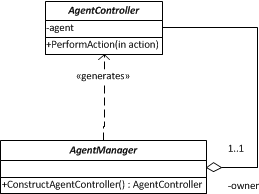
\includegraphics[width=0.7\textwidth]{AgentControllerDomainUML}
\par\end{centering}

\caption{Domain model for Agent Controller\label{fig:AgentControllerDomainModel}}
\end{figure}



\subsubsection{Concept}

The engine is designed to support the ability to be adapted for all
APL%
\footnote{Agent Programming Language%
} types, this means that the engine itself does not support all APLs
but instead provides a framework for quickly designing interfaces
between the engine and any APL. There are two classes that one must
use in order to properly design the interface:
\begin{description}
\item [{The~\texttt{AgentManager}}] has the duty of speaking directly
with the agent language it attempts to interface with. Its job is
to spawn an \texttt{AgentController} for each agent the AP wishes
to take control of. The \texttt{AgentManager} is in that sense much
akin to an Abstract Factory, which according to the design pattern
requires that an abstract class has a method generating a certain
type of what object but not exactly which object\texttt{\emph{ {[}rewrite
sentence{]}}}. The idea is of course that if you have a \texttt{GoalAgentManager}
then the controller it constructs would be \texttt{GoalAgentController}.
By making it an abstract method, we ensure at compile time that the
engine framework is properly used which is very good for the user.
\texttt{\emph{{[}Explain{]}}}
\item [{The~\texttt{AgentController}}] is the link between a single agent
and the AP %
\footnote{Agent Program%
}. Its job is to take all commands directed to it and transform them
into actions understood by the engine, and apply them to the agent
that it controls.
\end{description}
To simplify the \texttt{AgentController} design, it provides the method
\texttt{PerformAction}, which makes it easy to execute actions on
the agent it controls. When the \texttt{PerformAction} is called,
the \texttt{AgentController} queues the action given through the method
and puts the \texttt{AgentController}\textquoteright{}s thread to
sleep. Once the action has been executed by the engine, the \texttt{AgentController}
is woken up and returns from the \texttt{performAction} method. All
percepts received by the \texttt{AgentController} during this time
is stored on the \texttt{AgentController} and can be easily accessed
by the actual \texttt{AgentController}.

\begin{figure}
\begin{centering}
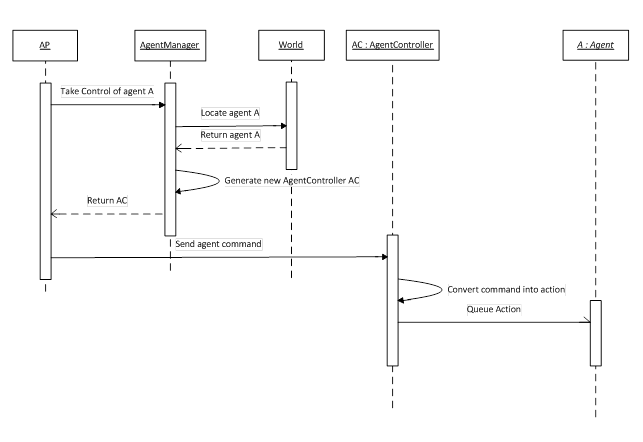
\includegraphics[width=0.7\textwidth]{SystemFeatureAgentControllerSequenceDiagram}
\par\end{centering}

\caption{This sequence diagram shows the process of an AP taking control of
agent through the \texttt{AgentManager}, and commanding it through
the \texttt{AgentController\label{fig:APConnectingToAndControllingAC}}}
\end{figure}


The process of an AP taking control of an agent is illustrated in
fig. \ref{fig:APConnectingToAndControllingAC}. The AP calls the \texttt{AgentManager}
to locate the agent it wishes to assume control of. The agent is located
through a string (its name) which is unique to it and ensures only
one agent is taken. When the \texttt{AgentManager} finds the correct
agent, it will immediately generate a new \texttt{AgentController}.
The AP will not gain access to the agent but instead it will gain
access to the \texttt{AgentController}. Now that the AP possesses
the \texttt{AgentController}, it will have the ability to send the
\texttt{AgentController} commands. These commands might not be understood
by the engine if the APL is foreign enough to the engine\textquoteright{}s
own language and as such it is the duty of the \texttt{AgentController}
to convert these commands into actual actions which the engine can
understand.

As this project is about working with GOAL in particular, we have
created an extension for the \texttt{AgentController} designed specifically
to work with GOAL. Therefore any example shown here would be incomplete
compared to the EIS/Goal implementation we have made. \texttt{\emph{{[}Remove
paragraph?{]}}}


\subsubsection*{Summary}

The agent controller is designed to be very lightweight, since we
do not want to impose any restrictions that might limit an APL which
we know nothing about. As such, the \texttt{AgentController} is more
akin to a convention or a design pattern for how interfacing with
agents should occur. It provides the skeleton of how a link might
be designed but does not impose any restriction of how should link
should be setup.
